We will generate new images using the tool TikZ. In subsequent classes, we will study Gnuplot and Inkscape.

\begin{figure}[h]
    \centering
    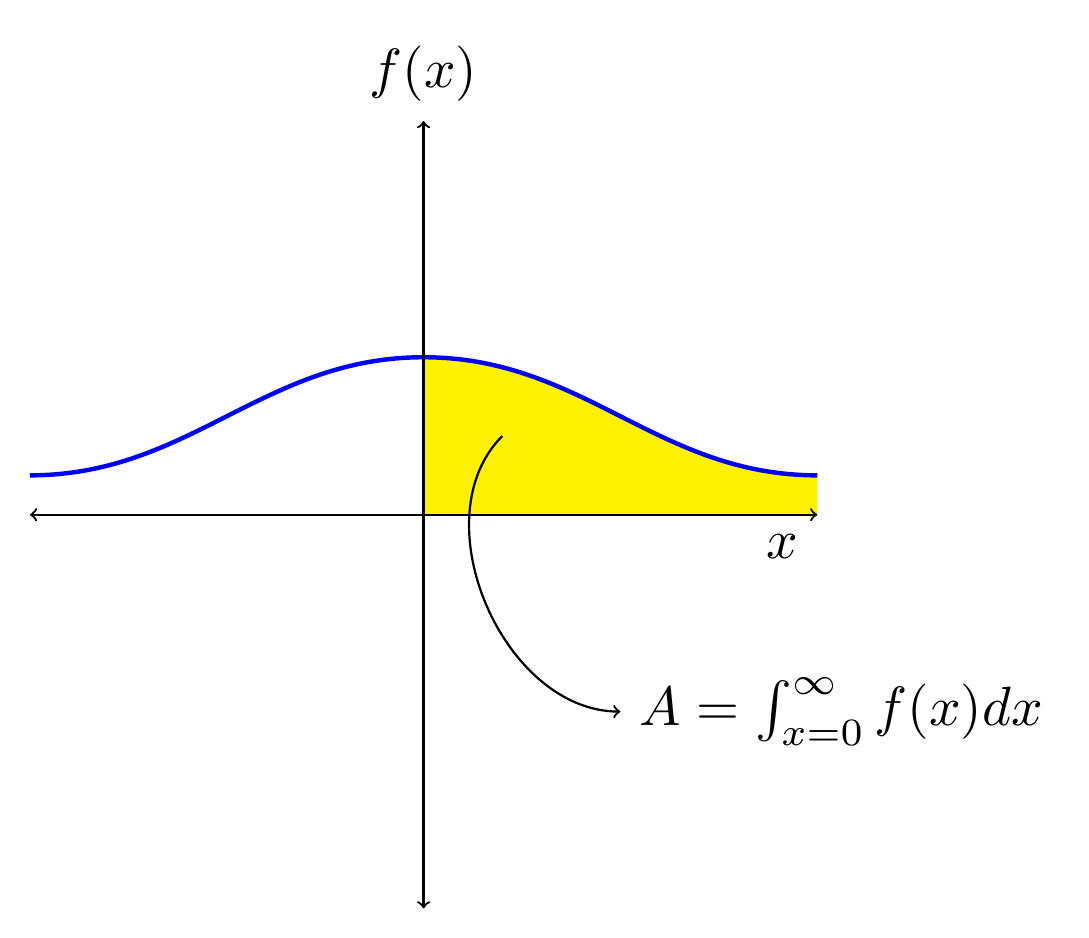
\begin{tikzpicture}[scale=0.5]
        %\draw [help lines] (-10,-10) grid (10,10);
        
        %\draw [red, fill=red, ultra thick] (4,4) circle [radius=.1];
        %\path [blue, fill=red, ultra thick] (-10,0) to [out=135, in=180] (0,5) to [out=0, in=45] (10,0) -- (-10,0);
        %\draw [red, domain=-4*pi:4*pi, line width=3pt, samples=50] plot (\x,{5*sin(\x r/2)});
        
        %\node [below right, scale=2] at (4,4) {A};
        
        
        %the main figure starts
        
        \path [fill=yellow] (0,4) to [out=0, in=180] (10,1) -- (10,0) -- (0,0) -- (0,4);
        \draw [blue, ultra thick] (-10,1) to [out=0, in=180] (0,4) to [out=0, in=180] (10,1);
        \draw [thick, ->] (2,2) to [out=-135, in=180] (5,-5);
        
        \draw [thick, <->] (-10,0) -- (10,0);
        \draw [thick, <->, rounded corners] (0,10) -- (0,-10);
        
        \node [below left, scale=2] at (10,0) {$x$};
        \node [above, scale=2] at (0,10) {$f(x)$};
        \node [right, scale=2] at (5,-5) {$A = \int_{x=0}^{\infty}f(x) dx$};
        
    \end{tikzpicture}
    \caption{Test Image}
\end{figure}